
\documentclass{sig-alternate}
\usepackage{hyperref}
\begin{document}
\conferenceinfo{WOODSTOCK}{'97 El Paso, Texas USA}
%\CopyrightYear{2007} % Allows default copyright year (20XX) to be over-ridden - IF NEED BE.
%\crdata{0-12345-67-8/90/01}  % Allows default copyright data (0-89791-88-6/97/05) to be over-ridden - IF NEED BE.
% --- End of Author Metadata ---
\title{IFuzzer: An evolutionary fuzzer using genetic programming}

\numberofauthors{3} 

\author{
\alignauthor
Spandan Veggalam\\
       \affaddr{IIIT Hyderabad,India}\\
       \email{
       veggalam.s@reseach.iiit.ac.in}
\and
% 2nd. author
\alignauthor
Satwik Bh\\
       \affaddr{IIIT Hyderabad,India}\\
       \email{
       satwik.bh@reseach.iiit.ac.in}
\and
% 3rd. author
\alignauthor
Sanjay Rawat\\
       \affaddr{IIIT Hyderabad,India}\\
       \email{sanjay.rawat@iiit.ac.in}
}

\maketitle

\begin{abstract}
Fuzzing is an automated black box testing used for finding security vulnerabilities in the software. Fuzzing generates well formed inputs and sends to application in order to hopefully trigger vulnerability. In this article we use evolutionary computing techniques in the area of interpreter fuzzing. The IFuzzer approach uses grammatical evolution techniques and guides the Fuzzer in generating well-formed codes that may trigger exceptional behaviour of Interpreter such as crashes, memory leaks, failing assertions. Fuzzed inputs must be syntactically valid to pass the interpreter elementary checks. The IFuzzer uses language grammar to generate random code fragments. IFuzzer is an effective tool applied on JavaScript interpreter found 22 vulnerabilities in the time span of one month.
\end{abstract}

\category{}{Security and Privacy}{Systems Security}[Vulnerability detection]
\terms{Security Testing}
\keywords{Security, Fuzzing, JavaScript, Grammatical Evolution, Evolutionary Algorithm, 
Artificial Intelligence, Web Applications, Interpreters}

\section{Introduction}
\indent Software security is essential dimension for a software. Web browser are one of the application software serves as an interface for computer networks and many computer systems. These browsers are becoming more and more sophisticated, their by render different services for which they include several interconnected components. Interpreters are of one such component for languages like JavaScript, PDF, Php, XSLT and many more. Because of their widespread usage, they became primary applications for security attack, data and privacy breaches. The interpreters included can be exploited for launching browser based security attacks. JavaScript is one such widely used interpreter responsible for several vulnerabilities. We look at such attacks in the following perspective:
\begin{enumerate}
\item The way of handling information which includes extracting, parsing, storing, manipulating and communicating may also raise some vulnerabilities.
\\e.g., Cross Site Scripting
\item Flaws in browser software components like script engines, plug-ins, etc., can be used to exploit vulnerabilities. 
\item Browser components may also result in low-level vulnerabilities which can be exploited.
\\e.g., memory corruptions, assertion failures, uncommon behaviours etc.
\end{enumerate}
\indent The Web has proved to interlink different information systems and has become main medium for sharing information. In the recent past, there have been numerous studies, techniques, and tools proposed mainly to address the security issues related to information processing.	However, in the context of web related vulnerabilities particularly software's like browsers and their components, not much has been investigated in the direction of the above mentioned point 2. As a result, recently, there have been many bugs uncovered in browser-run software's: e.g., Spidermonkey, Firefox JavaScript Engine.\\
\indent Fuzz testing is a useful approach for finding vulnerabilities in software. One of its variants, evolutionary fuzzing, turned out to be a useful smart fuzzing method. These methods make use of evolutionary computing approaches to automatically generate inputs that exhibit vulnerabilities.\\
\indent Interpreter fuzzers must generate syntactically valid input, otherwise inputs will not pass the elementary interpreter checks. Therefore input must be generated making use of knowledge about target language. Assuming JavaScript interpreter to be target, fuzzed input must follow the syntax rules of JavaScript. Otherwise JavaScript interpreter discards the inputs during its first step i.e., parsing. Therefore JavaScript language grammar is used to generate syntactically valid code fragments. With built-in language grammar valid data can be modelled. Both language dependent and independent fuzzer can be built with some additional knowledge of a specific language. \textit{jsfunfuzz} is popular fuzzer for Mozilla's JavaScript engine. This is an example for language dependent fuzzer. Another fuzzer \textit{Langfuzz} is an example of language independent fuzzer generates syntactically valid code fragments. With the motivation from this language independent fuzzer - can we map langfuzz approach to genetic programming paradigm?\\
\indent In this paper we will introduce a new framework called \textit{IFuzzer}, that generates code fragments using Grammatical Evolution methods (particular form of Genetic Programming), thereby allows black box fuzzing of the Interpreters. IFuzzer takes context free grammar as input, for instance given JavaScript grammar it generates JavaScript programs; uses grammar to learn code fragments from the input code base. Given a test suite, IFuzzer performs standard Gentic Algorithm  operations; crossover and mutations on the input code fragments and uses learnt code fragments for replacements - Grammatical Evolution brings transparency on making decision, inspired by biological evolution. It follows Darwin's theory of evolution and selects programs with high fitness. Here, Fitness function favours  the program which are uncommon enough and likely to trigger interpreter exceptional behaviours and are selected for fuzzing. Grammatical Evolution approach is appropriate at generating code, and likely to produce diverse code fragments.
\begin{figure*}
\centering
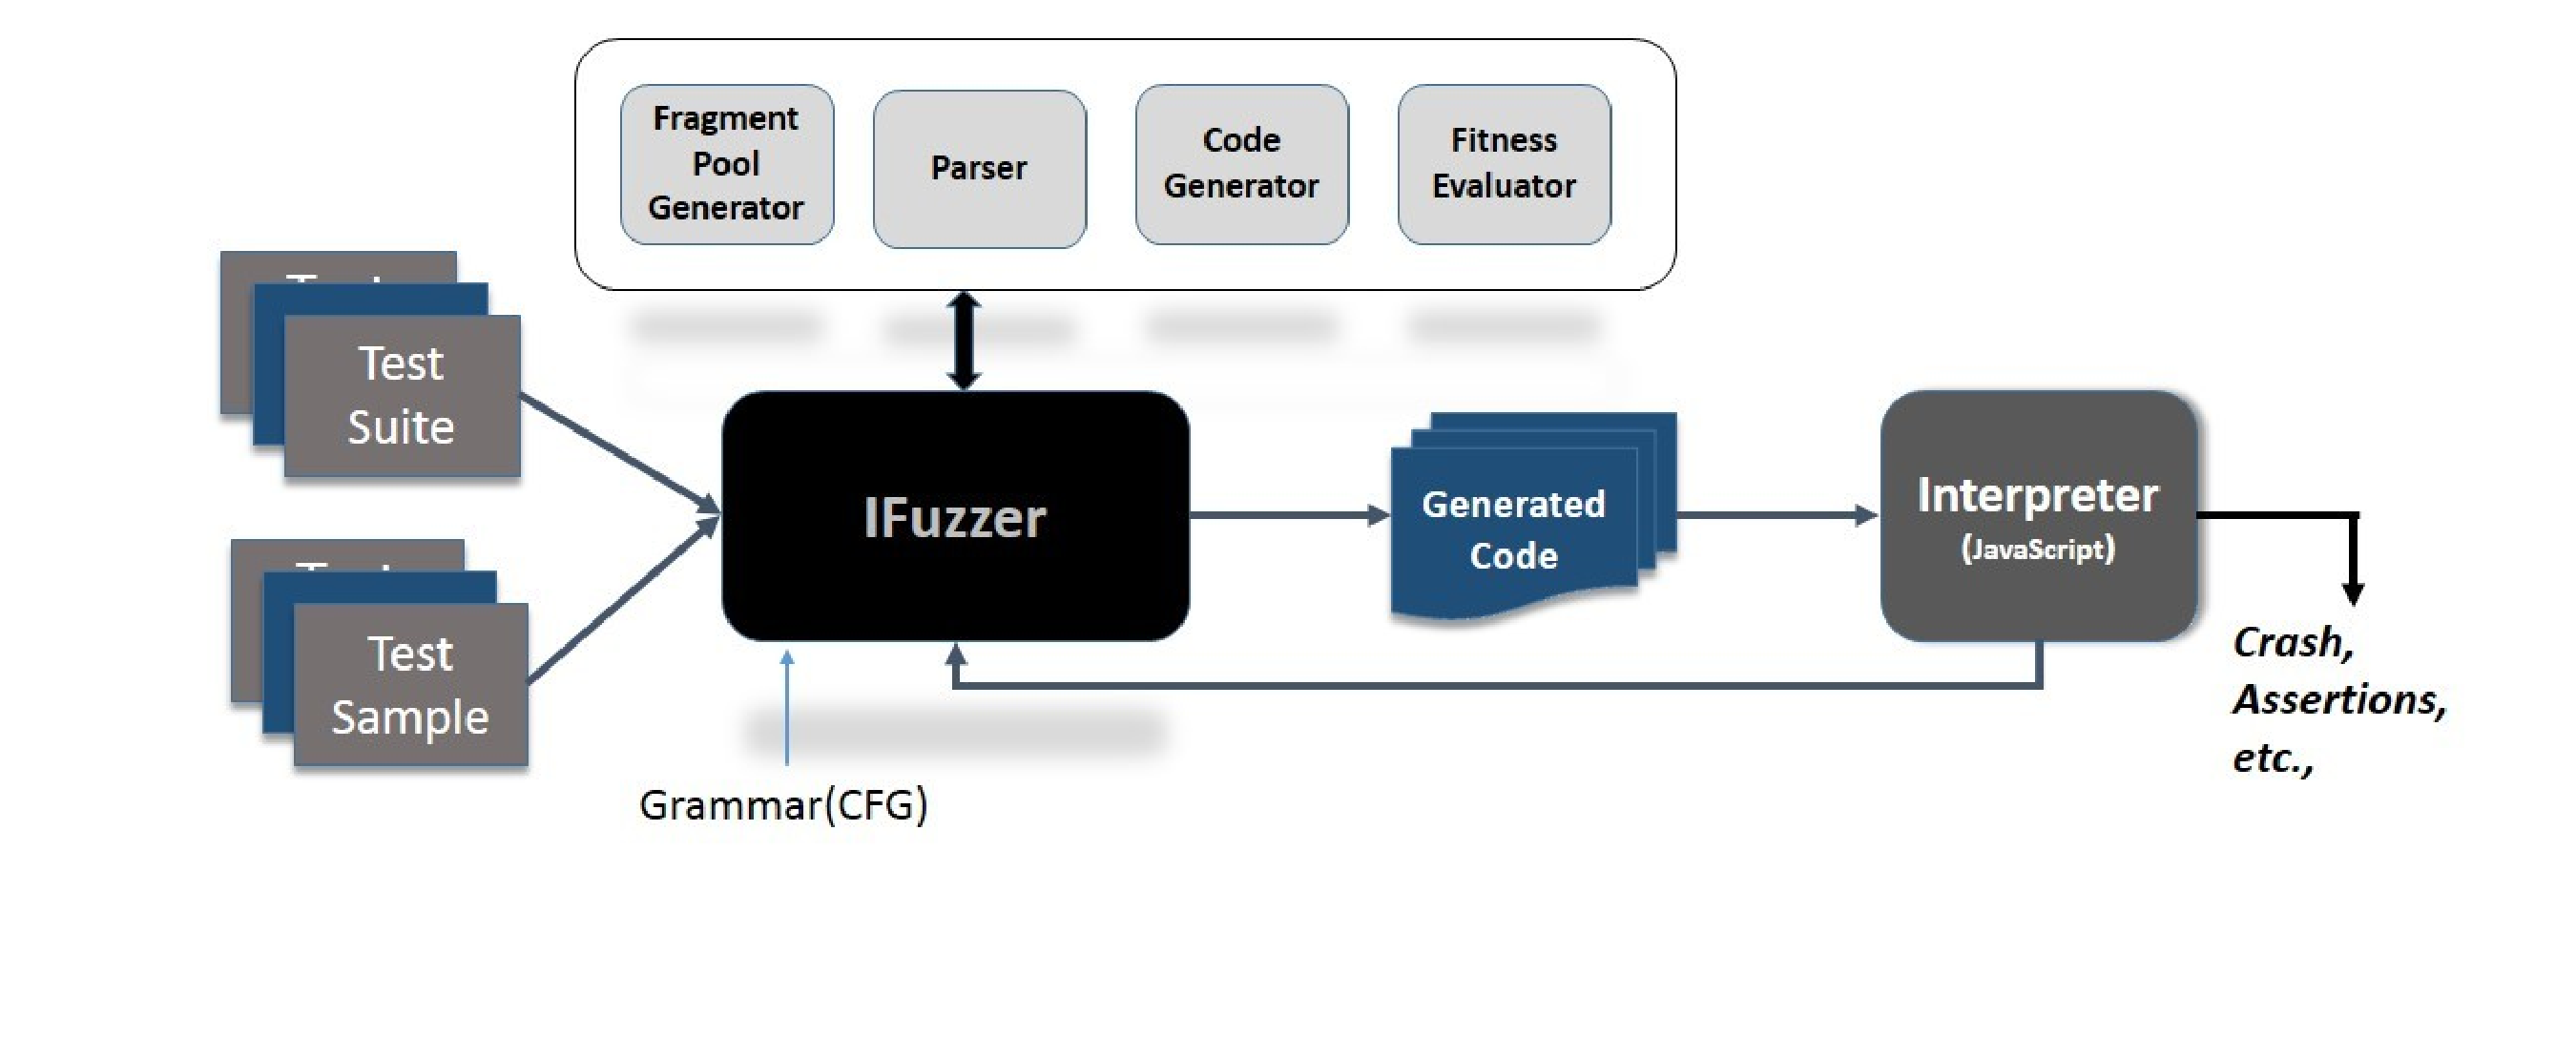
\epsfig{file=process.eps, height= 2.8in, width=6.5in}
\caption {Overview of IFuzzer Approach}
\medskip
 describes the overview of IFuzzer which takes test suite, language grammar and sample code as input. Language grammar is used to parse the program. Parser uses language grammar to parse the program and generates 
\label{fig1}
\end{figure*}
\\\indent  Figure \ref{fig1} describes the overview of IFuzzer which takes test suite, language grammar and sample code as input. Language grammar is used to parse the program. Parser uses language grammar to parse the program and generates XML object as abstract syntax representation. Fragment pool of code fragments formed by parsing each input file from sample codes. Test suite itself can be used as sample codes. IFuzzer generates new code fragments by performing genetic operations on the test suite. 
\\Remaining paper explains the code generation process and fuzzing process. ~\autoref{sec:bk} presents the motivation for choosing Grammatical Evolution for code generation. In ~\autoref{sec:GEIF} we describe the methods involved in code generation process. Implementation of IFuzzer is discussed in ~\autoref{sec:impl}.
\section{Motivation} \label{sec:bk}

\subsection{Terminology}
\indent In the following sections we make use of following terminology.
\begin{enumerate}
\item{\textbf{Interpreter.}} In this paper the term \textit{"Interpreter"} is software system that executes input program. This translates code from one form to other form during execution. 
\item{\textbf{Genotype.}} In this paper the term \textit{"Genotype"} refers to the structural representation of the program which is operated on by crossover and mutation
\item{\textbf{Phenotype.}} In this paper the term \textit{"Phenotype"} refers to the structure of the program that is  directly executed and on which fitness is calculated based on the behaviour of this individual.
\item{\textbf{Grammar.}} The grammar defines the context free grammar of the target language. Grammar is defined in Backus Normal Form or extended Backus Normal Form.
\item{\textbf{Genome.}} Linear Representation of an individual in Grammatical Evolution is Genome.Genomes are used in selecting different productions rules during code generation process.
\item{\textbf{Codon.}} \textit{Codon} is building block of Genome. Each codon is of equal size. 
\item{\textbf{Bug/Defect.}} In this paper the term \textit{bug} or \textit{defect} refers to an abnormal behaviour of the target software system (e.g. Crash due to memory overflows, assertion failures, etc.) 
\end{enumerate}

\section{IFuzzer Approach} \label{sec:GEIF}
\indent In this section we discuss how to use Grammatical Evolution(GE) Techniques for program generation. In general testing inputs are generated using Generative approaches or Mutation approaches or both. \textit{IFuzzer} makes use of both mutation and generative approaches. IFuzzer follows Grammatical evolution approach in code generation. Grammatical Evolution is a Genetic Programming(GP) paradigm and analogous to biological evolutionary process. Grammatical Evolution applies genetic operators crossover, mutation and replacements on the individuals in program generation process. 

\subsection{Representation}
\indent Genetic programming and Grammatical Evolution differs in the way the inputs are represented. GP confined to use tree structures for program representations. Various variants of GP are proposed based on program representations. GE doesn't pose any constraints on structure generally follows linear representations like strings, binary string etc., IFuzzer follows binary string representation of the programs which is referred as genome. All the genetic operations are performed on the genome and are applied on the program.  In binary representation genome is sequence of bits generated randomly. For eg., variable statement \textit{var s;} is represented in binary representation as follows.
\begin{center}
var s;
\\1100110101010111100100111101001001010110
\end{center}

\subsection{Fragment Pool}
\indent From the set of files code from input code base fragment pool is formed by extracting code fragments for each non terminal in the language grammar. In this phase, we process each input file by the language parser. Using the parser, code fragments are extracted from the input files. Each code fragment is represented by a non-terminal. With sufficient number of input files, code fragments can be generated to all non-terminals in the language grammar. These code fragments are used in mutation and code generation phase, same logic is followed in crossover for identifying code fragments for selected common non-Terminal between the participating individuals\\
\indent In mutation code fragments in the input is replaced with corresponding non-terminal code fragment selected from the fragment pool. In crossover code fragments of same type from two different programs are exchanged with each other. All these operations may be semantically invalid  or not useful in the context of input programs involved in different phases. For this we perform semantic improvement and new code fragments are generated in context of participating individual semantics

\subsection{Initial Population}
\indent A set of initial population of individuals are generated by randomly selecting certain number of programs equal to population size from the input test samples. This forms first generation of evolution. After each generation individuals forms the parental set of individuals(Genotypes) which undergo genetic operations, and their by evolves into off-springs enforcing to maximum size of population.

\subsection{Genetic Algorithm Operations}
\subsubsection{Crossover}
\indent In GE crossover is analogous to biological operation, performed on string based linear structure(Genome) and is considered to be an explorative operator. Types of crossover operations are differentiated based on number of crossover points. In our approach we perform  homologous two point crossover on two individuals by swapping code fragments that belongs to same non-terminal. Following steps are followed:
\begin{enumerate}
\item Parse the two individuals that undergo crossover by the language parser. \item Identify list of common non-terminals based on set of code fragments that can be formed from the individuals.
\item A non-terminal is randomly selected from the list of common non-terminals. 
\item Code fragment of common non-terminal is randomly selected from both the individuals is exchanged with each other. More than one code fragment in an individual may be an example of selected common non-terminal.
\item Typically 1..3 non-terminals are randomly selected (for crossover) in this process. 
\end{enumerate}

\subsubsection{Mutation}
\indent Mutation brings diversity among the population by replacing code fragment with different code fragments of same type. For this we pick some of code fragments randomly from the fragment pool and replace them with the code fragments of same type. Before replacing them directly, we perform some improvements as discussed in ~\autoref{sec:cgen} and replace code fragment with the one formed by expanding the non-terminal using the corresponding production rules from language grammar and replacing the code terminals for the non-terminal that represents the code fragment selected for mutation. Typically mutation is performed by randomly selecting 1..3 non-terminals.

\subsubsection{Replacement}
\indent During the process of off-spring generation, it is important to retain the features of best chromosomes (parents) participating in evolution. Therefore Fitness elitism method is followed to retain the best chromosomes among the parents, and these chromosomes are included as the off-springs. Remaining off-spring population is formed with the ones generated from crossover and mutation. This prevents the loosing the best ones in the process.

\subsection{Code Generation} \label{sec:cgen}
\indent With Crossover and Mutations, we generate diverse code fragments and order of genetic operations is purely random either of mutation or crossover can take place first. \\
\indent Using language parser parses the input program and returns the abstract syntax tree represented by an XML structure. Tags in XML object are formed with language non-terminals and text embedded between tags is the code fragment identified from input program according to language syntax. All the non-terminals nested and ordered according to input program structure. Extracting the text in the order of XML structure re-generates input program itself. \\
\indent During mutation method, several random code fragments part of input program are selected for mutation. Removing the selected non-terminal form an incomplete program and voidness of this code fragment is filled by code fragment that can be identified by non-terminal or non-terminal is expanded to complete program. We use following expansion algorithm:
\begin{enumerate}
\item Following steps are executed in loop     upto a depth \textit{d}
\begin{enumerate}
\item Set of non-Terminals in the incomplete program are identified.
\item Identify the set of productions $P_{n}$ $\subset$ P under the non-Terminal \textit{n}.
\item Modulo operation on the number of productions with decimal integer of codon, a production \textit{p} is selected. 
\[p_{rule-selected} = codon mod number-of-rules\]
\item Replace the non-terminals occurrence with \textit{p}.
\item Gene string is appended to itself in case of in sufficient codon values.
\end{enumerate}
\item After expanding to a certain depth \textit{d}, all the remaining non-terminal occurrences are to be replaced with terminals to yield complete program. For this we randomly select same type of code fragments from fragment pool.
\end{enumerate}
\indent \textit{Codons} are the chunks of 8-bits from the gene of the individual.\\
\indent In Crossover, several random fragments (Typically 1..3) are selected from the both the individuals by selecting common non-terminals from the corresponding XML objects. These selected fragments from one individual are exchanged with fragments of other individual. All these operations are performed on XML objects, after which new programs are generated from these modified XML objects.\\
\indent Genetic operators mutation or crossover or both performed on the population in each generation and thereby forms off-spring population i.e. next generation. Code generation process is continuous process and is terminated after a certain number of generations or based on stopping criteria. \\
\indent With primary target to trigger exceptional behaviour of the Interpreters and Compilers, we start with existing test cases written for the target language by developers as a standard practice. All the  processes discussed above are applied to the test cases one after one, from the learning phase to mutation phase, thereby creating executables from the original test cases.

\subsection{Semantic Adjustment} \label{sec:semantics}
\indent In our Language Independent approach, we try to generate semantically valid programs by maintaining semantical context of the input programs. Introducing language semantics ties IFuzzer to a language specifications. Code fragments generated with Crossover, Mutation and Initial Population generation   methods might be semantically invalid or out of semantic context of original inputs. We perform generic class of semantic transformations as part of small semantic adjustments at syntactic level. \\
\indent Continuation of semantics is one such generic approach can be used to any programming language. Re-using literals occurred in body of input programs is an example of this approach. With this we can reducing undeclared identifier exceptions. In most of the languages all the memory locations and functions are named with identifiers and are declared somewhere in the body of the program. These identifiers must be declared before they are used, but in some languages like JavaScript they can be declared anywhere in the program and are evaluated during run time. Re-using the identifiers from the body of the original input within the new fragments reduce the chances to have undeclared identifiers. This can be done at the syntactic level. For this IFuzzer need to know the identifiers used in the input program, from the language grammar using identifier non-terminal we identify the identifiers from the program and replace identifiers in new fragments. It is still possible that identifiers are undeclared at the time of executing (because the reused identifier may be declared downward the new fragment) but the chance of undeclared identifier is reduced. \\
\indent IFuzzer is aware of the language global objects and built in functions which can be used with out declaring them. List of these objects and functions are passed as an argument with which they are identified in the new fragments. These objects are left unmodified by IFuzzer, are usually defined in the implementation of language.

\section{Implementation} \label{sec:impl}
\indent A fuzzer is implemented as proof-of-concept based on all the methods discussed so far and works as described in overview diagram (Fig. 1) in the introduction. IFuzzer starts with Fragment Pool generation process, where it takes each input file from the test suite and extracts code fragments for different non-terminals in language grammar.
After extracting fragments from all input file, fuzzer starts it code generation and fuzzing process.

\subsection{Parsing}
\indent In most of the discussed methods input code is parsed and corresponding XML structure is generated. For this, IFuzzer uses ANTLR parser generator framework to generated parsers for different languages using grammar specified in BNF. We decided to use ANTLR because of different parser generation options, and it has grammars for several languages. Parser is used to extract code fragments from input test suite or to generate abstract syntax for which in either cases parser generates XML object as abstract syntax of program. Code fragments are extracted for each non-terminal from these XML objects. XML objects are involved in fragment pool generation and code generation methods.

\subsection{Code Generation}
\indent IFuzzer uses ANTLR parser for target language which generated using ANTLR language grammar. As discussed in ~\autoref{sec:cgen} Crossover, Mutation and Initial Population generation methods make use of XML objects returned by the parser for performing their operations. Small simplifications are made to grammar syntax internally without making any semantic changes and also changes are made to introduced Identifier as non-terminal (In most of ANTLR grammars identifier is included as terminal fragment). This makes step-wise expansion algorithm discussed in ~\autoref{sec:cgen} easier and newly introduced identifier non-terminal simplifies semantic adjustment and identifiers listing process. 
\indent Grammar simplification includes following modifications:
\begin{enumerate}
\item Rules containing sub-alternatives are written as separate rules.
\item All the rule quantifiers and optionals are removed by introducing additional rules.
\end{enumerate}
Additional rule created are added to corresponding non-terminals. After these simplifications all the rules are left with non-terminals and terminals.\\
\indent During Initial population creation itself, identifiers are extracted for particular individual and cached for further processing. In Code generation process, new fragments are fitted into existing semantic-al context as explained in ~\autoref{sec:semantics}. For this purpose IFuzzer uses the cached identifiers for replacing the identifiers in new fragments. For suppose if an identifier "a" in new fragment is replaced with "b", all the occurrences of "a" are replaced with "b". Local Identifiers are mapped to Global and built-in identifiers but vice versa will not happen.\\
\indent Code generation process is continued for a number of generations or until a individual with target fitness value is generated. 


\subsection{Fitness Evaluation} \label{sec:fitness}
Individual's fitness is calculated at different stages. After crossover and mutation phases generated the code fragments are evaluated. Fitness value is calculated based on different factors. Various program parameters which includes structure of program, warnings raised by the interpreter, crashes, execution time outs, singularity are considered as fitness parameters. For instance nested (or complex) structure have tendency to create uncommon behaviour, so it gains more score compared to less complex structured programs. Entire evolutionary process is an objective driven process therefore fitness plays an vital role in code generation process. 

\subsection{Executing tests}
IFuzzer executes the test inputs generated after each GA methods discussed. Valid test cases are considered for fitness evaluation. IFuzzer requires to generate more number of population generations thereby and after each iteration code generation moves towards the more objective function. Here the objective is to identify uncommon behaviour of interpreter with valid inputs. All the tests are performed in the persistent shell of the interpreter and uncommon behaviours are traced. \\ 
\indent IFuzzer contains many adjustable grammatical evolution parameters, e.g. mutation rate, crossover rates, population size, number of generations and many others. All the default values are derived from experiments. We tried to use the best combination based on observations, but these doesn't promise the certainty to deliver the best performance. It is not feasible to compare all parameter combinations because the evaluation of parameter set is time consuming. Repeating the process several times and observing the process to compare the results is not practical to do easily. In Table 3 (see appendix) we listed the important parameters and their default values.\\
\indent  Delta Debugging algorithm is used to filter out the irrelevant code from the test case resulting in small test cases, thereby part of test case that is relevant to failure is filtered out. This algorithm reduces the number of lines of code executed and  results in suitably small code fragment that causes failure.


\section{Evaluation}
\section{Related Work}
\section{Conclusion}


\end{document}
